\documentclass[onecolumn, draftclsnofoot,10pt, compsoc]{IEEEtran}
\usepackage{graphicx}
\usepackage{url}
\usepackage{setspace}

\usepackage{listings}
\usepackage{xcolor}
\usepackage{float}

\usepackage{geometry}
\geometry{textheight=9.5in, textwidth=7in}

\usepackage{hyperref}
\hypersetup{
    colorlinks=true,
    linkcolor=blue,
    filecolor=magenta,      
    urlcolor=cyan,
}

\makeatletter
\renewcommand\paragraph{\@startsection{paragraph}{4}{\z@}%
            {-2.5ex\@plus -1ex \@minus -.25ex}%
            {1.25ex \@plus .25ex}%
            {\normalfont\normalsize\bfseries}}
\makeatother
\setcounter{secnumdepth}{4} % how many sectioning levels to assign numbers to
\setcounter{tocdepth}{4}    % how many sectioning levels to show in ToC


\definecolor{lightgray}{rgb}{.9,.9,.9}
\definecolor{darkgray}{rgb}{.4,.4,.4}
\definecolor{purple}{rgb}{0.65, 0.12, 0.82}

\lstdefinelanguage{JavaScript}{
  keywords={typeof, new, true, false, catch, function, return, null, catch, switch, var, if, in, while, do, else, case, break},
  keywordstyle=\color{blue}\bfseries,
  ndkeywords={class, export, boolean, throw, implements, import, this},
  ndkeywordstyle=\color{darkgray}\bfseries,
  identifierstyle=\color{black},
  sensitive=false,
  comment=[l]{//},
  morecomment=[s]{/*}{*/},
  commentstyle=\color{purple}\ttfamily,
  stringstyle=\color{red}\ttfamily,
  morestring=[b]',
  morestring=[b]"
}
 
\urlstyle{same}

% 1. Fill in these details
\def \CapstoneTeamName{		ConnectBasket Development Team}
\def \CapstoneTeamNumber{		39}
\def \GroupMemberOne{			Henry Fowler}
\def \GroupMemberTwo{			Kailyn Hellwege}
\def \GroupMemberThree{			Taylor Kirkpatrick}
\def \CapstoneProjectName{		ConnectBasket}
\def \CapstoneSponsorCompany{	OSU MIME}
\def \CapstoneSponsorPerson{		Dr. Chinweike Eseonu}

% 2. Uncomment the appropriate line below so that the document type works
\def \DocType{		%Problem Statement
				%Requirements Document
				%Technology Review
				%Design Document
				Final Report
				}
			
\newcommand{\NameSigPair}[1]{\par
\makebox[2.75in][r]{#1} \hfil 	\makebox[3.25in]{\makebox[2.25in]{\hrulefill} \hfill		\makebox[.75in]{\hrulefill}}
\par\vspace{-12pt} \textit{\tiny\noindent
\makebox[2.75in]{} \hfil		\makebox[3.25in]{\makebox[2.25in][r]{Signature} \hfill	\makebox[.75in][r]{Date}}}}
% 3. If the document is not to be signed, uncomment the RENEWcommand below
\renewcommand{\NameSigPair}[1]{#1}

%%%%%%%%%%%%%%%%%%%%%%%%%%%%%%%%%%%%%%%
\begin{document}
\begin{titlepage}
    \pagenumbering{gobble}
    \begin{singlespace}
    	
\includegraphics[height=4cm]{coe_v_spot1}
        \hfill 
        % 4. If you have a logo, use this includegraphics command to put it on the coversheet.
        %\includegraphics[height=4cm]{CompanyLogo}   
        \par\vspace{.2in}
        \centering
        \scshape{
            \huge CS Capstone \DocType \par
            {\large\today}\par
            \vspace{.5in}
            \textbf{\Huge\CapstoneProjectName}\par
            \vfill
            {\large Prepared for}\par
            \Huge \CapstoneSponsorCompany\par
            \vspace{5pt}
            {\Large\NameSigPair{\CapstoneSponsorPerson}\par}
            {\large Prepared by }\par
            Group\CapstoneTeamNumber\par
            % 5. comment out the line below this one if you do not wish to name your team
            \CapstoneTeamName\par 
            \vspace{5pt}
            {\Large
                \NameSigPair{\GroupMemberOne}\par
                \NameSigPair{\GroupMemberTwo}\par
                \NameSigPair{\GroupMemberThree}\par
            }
            \vspace{20pt}
        }
        \begin{abstract}
        % 6. Fill in your abstract    
        

        \end{abstract}     
    \end{singlespace}
\end{titlepage}
\newpage
\pagenumbering{arabic}
\tableofcontents
% 7. uncomment this (if applicable). Consider adding a page break.
%\listoffigures
%\listoftables
\clearpage

% 8. now you write!

\section{Introduction to Project}

\subsection{Project Purpose}
This project will create a web application called ConnectBasket that will serve as a new tool for the Oregon State University Veterinary Hospital to improve communication within the hospital and externally with patient owners and other hospitals. The current workflow in the hospital involves receptionists taking calls, typing a message into the system, printing out that message, and walking it across the hospital to a veterinary technician or doctor to look at and add a handwritten note to. After that, the doctor or technician will carry the message to another doctor or technician, or back to reception or scheduling, who will call the initial caller and answer the question they had or schedule an appointment for them. The main purpose of this project is to eliminate the paper aspects of this process and make an electronic system that allows messages to be created and sent to other employees of the hospital, and notes to be added to those messages. It will then be able to display messages back to users with all of their associated notes. This project will help increase the efficiency of communication at the hospital as well as provide a less error-prone system that allows users to see a complete history of all messages.

\subsection{Project Goals}
\begin{itemize}
\item Allow users to create a message which will be associated with a patient and an owner of that patient
\item Allow messages to have a status to tell whether they are open or closed
\item Allow messages to be routed to other users or groups of users
\item Allow notes to be added to messages
\item Allow users to select a group or groups to be a part of
\item Provide an audit log of all messages created over a given time period
\item Increase the overall efficiency of messages being transported throughout the hospital 
\item Reduce the amount of paper being printed
\item Reduce errors in the communication process of the hospital 
\end{itemize}

\subsection{Clients}
The official client was Dr. Chinweike Eseonu, a professor in the College of Engineering at Oregon State University. The other client was Kelly Warner, the Process Improvement Manager at the Oregon State University Veterinary Hospital.

\subsection{Development Team}
All parts of the project were discussed and planned by all members of the team, but each team member had specific parts of the project they focused on. Most features of the website were a result of contribution from multiple team members.

\subsubsection {Henry Fowler}
Henry focused on the database and back end of the project. Designing and creating the tables and stored procedures stored in the MySQL database and writing the PHP code to interact with the database from the website.

\subsubsection {Kailyn Hellwege}
Kailyn was responsible for most of the front end development of the website. Writing the HTML and CSS that style all of the pages of the site and the Javascript code that makes the pages dynamic.

\subsubsection {Taylor Kirkpatrick}
Taylor designed and created the notification system for the website, including the shell script responsible for sending the notifications. He also worked on setup and configuration of the web server that the website is running on.

\subsection{Role of the Clients}
Dr. Eseonu provided some guidance and suggestions about overall design and features of the project. Kelly provided most of the input into what the website should look like and what features were needed.

\newpage
\section{Requirements Document}
\subsection{Introduction}

\subsubsection{Purpose}
The purpose of this document is to outline the requirements for an improved communication system for the Oregon State University (OSU) Veterinary Hospital, called ConnectBasket. 
This document's audience is the client, as well as certain staff members at the hospital. This document will be used as a way to measure the success of the Capstone development team working on this project. 


\subsubsection{Scope}
ConnectBasket will be a web based portal for the OSU Veterinary Hospital that will streamline the way messages are moved around the hospital and provide a better way to track the route that messages have taken. When an owner calls the hospital, receptionists will be able to type a message into the computer, assign it a category, and route it to the necessary staff members, which may be service specific vet techs, house officers, or faculty. Those staff members will be alerted, either by email or text, that they have a message waiting for them in ConnectBasket, and once viewed, notes can be added and the message can be re-routed to other staff members. After a message has been addressed by the necessary staff, the message can be closed, meaning no more notes can be added. The audit trail of when the message was created and closed will be visible, along with all the notes, timestamps of notes, and staff who added the notes.


\subsubsection{Definitions, Acronyms, and Abbreviations}
\begin{itemize}
\item Capstone - CS 461 class at Oregon State that the developers of ConnectBasket are in
 
\item OSU - Oregon State University

\item Hospital - referring to the OSU Veterinary Hospital

\item Owner - a person who owns a pet that is a client of the hospital

\item Patient - an animal who has/is going to be treated at the hospital 

\item VetHosp - the hospital management system used by the OSU Veterinary Hospital for keeping patient and owner records

\item Mobile Devices - smartphones or tablets
\end{itemize}
\subsubsection{References}
IEEE Std 830-1998, IEEE Recommended Practice for Software Requirements Specifications

\subsubsection{Overview}
The second section of this document will contain a further description of the ConnectBasket project, including product functions, user characteristics, and constraints. The third section will define the specific requirements of the project. 

\subsection{Overall Description}

\subsubsection{Product Perspective}
The ConnectBasket web based portal will be a stand alone system that will have additional functionality to connect to the current VetHosp system used by the hospital. ConnectBasket will use patient and owner information stored in the VetHosp system to connect information collected with the correct patients and owners, given that access to the data in VetHosp is provided to the Capstone development team.

\paragraph{User Interfaces}
There will need to be some level of security requiring users to login to access the information in the system. The system will provide users with the ability to search for a patient or owner and to enter new messages for them as well as view older messages and the audit trail associated with the message.

\paragraph{Hardware Interfaces}
Staff will be able to access the system from their desktop or laptop computers as well as mobile devices.

\paragraph{Software Interfaces}
ConnectBasket might be able to interface with the VetHosp program in order to connect information collected with the information about patients and owners stored in VetHosp. Access to the patient and owner information stored in VetHosp will be required for a system that could be integrated with VetHosp.

\subsubsection{Product Functions}
\paragraph{User Stories}
The receptionists at the hospital will need to be able to take calls from owners, enter a message into ConnectBasket, and forward it on to necessary staff members, such as vet techs or doctors. After that, the staff receiving the message can perform the action requested of them, and add any notes to the message. Then, it can be rerouted to other staff members. At the end of the chain, the message will be routed back to scheduling or reception, where they can contact the owner with information or to set up an appointment. They will then mark the chain as closed, and it will be able to be viewed later by staff members with permission to view audit logs.
\paragraph{Function Dependencies}
See Original Gantt Chart.

\subsubsection{User Characteristics}
Users of ConnectBasket will be staff members of the hospital. The users will have a variety of different education levels and experience. Therefore, the system will need to be designed so that technical expertise is not required in order to properly use it.

\subsubsection{Constraints}
The performance of the ConnectBasket application will be limited by a staff member's internet connection. Staff should not use the service on unsecure networks, as messages sent with it should have some degree of confidentiality due to the nature of the work, the hospital's policies, and government regulations. This limits where the application can be accessed from, as non-trusted networks may expose these messages. Staff may also only access this application with a verified user account.

\subsubsection{Assumptions and Dependencies}
It will be assumed that staff will not be attempting to use non-English languages for messaging. This system might depend on the hospital's existing VetHosp software, and integration with it is a goal for this project. Integration will depend on the VetHosp software being available to the developers and the level of access the Capstone development team will have to it. VetHosp integration will also depend on the hospital's IT team arranging an integration of ConnectBasket with VetHosp. Any changes that need to be made to the VetHosp system for integration will need to be done by the team in charge of developing VetHosp, not the Capstone development team. However, ConnectBasket will be capable of operating independently without any integration.

\subsection{Specific Requirements}

\subsubsection{External interface requirements}

\paragraph{VetHosp}
ConnectBasket might be integrated with VetHosp as it nears completion, so that it can pull information from VetHosp as needed to populate fields and reduce separate instances of data lookup. Detailed information about VetHosp is not currently available to the development team, and successful integration will depend on the level of access provided to the Capstone development team.

\subsubsection{System features}

\paragraph{Creation of Messages}
ConnectBasket will allow receptionists to create messages and route them to other parts of the hospital. Receptionists and other staff should be able to route messages with patient information to the relevant locations in the hospital. These messages should be secure and not exposed to public channels, and may need to be encrypted as well.

\paragraph{Message Auto Population}
ConnectBasket will allow message composers to easily write messages by auto populating some fields of the message, such as the current date and patient and owner names. By auto filling and not allowing free text for certain fields, message creation will be more efficient and less error-prone. These fields will be prefilled for convenience and to send off messages quicker and in a standard format. This feature will also include utilizing drop-down menus instead of plain text to reduce error for other fields, such as recipients of messages and category of messages.

This feature will be useful for both convenience and safety, as constraining messages to at least some pre-defined standard will reduce the likelihood of human error in medical situations.

\paragraph{Message Notification}
ConnectBasket will send message recipients notifications when a message has been routed to them or a category their profile belongs to. Notifications will be delivered as a text message, email, or both, depending on the preferences of the staff member. Staff members will have the option to receive alerts simply after a message is received or after a message is unread for a portion of time.

\paragraph{Message Review and Forwarding}
ConnectBasket will allow message recipients to review their messages online via any internet-accessible device, should the connection or other factors not restrict them from doing so. Staff who have viewed a message will be capable of rerouting this same message to other necessary staff, along with any comments or addendums added by the previous recipient. 

\paragraph{Message Resolution}
ConnectBasket will allow message recipients to resolve messages as closed, should the task or job mentioned within it be completed. This closed state should remove the message from all staff member's queues, allowing them to focus on other tasks that have not been resolved.
	
Ideally, this feature will include more than just a closed state; it will include additional states that show other reasons for a task to no longer be active, such as cancelled, duplicate, or stopped, to provide more information about the status of a task.

\paragraph{Message Audit Record}
ConnectBasket will allow staff with sufficient permissions to view a message's  history for audit or review. Authorized staff will  be able to see when and where the message was created, when and where it was routed, and when and where it was closed. The name of any staff member who took any action should also be recorded, along with other activity regarding a message. 

Providing an audit trail for all messages will provide the hospital with valuable information and allow them to track metrics such as the average amount of time the hospital takes to respond to calls and common reasons for owners calling the hospital. 

\paragraph{Message Recipient Roles and Profile Roles}
ConnectBasket will allow staff to select and be assigned to one or more roles that reflect their duties and responsibilities at the hospital. Staff will have profiles to manage their roles, with the ability to change their roles at will. When messages are routed to a specific department, any staff member that has selected the associated role to that department will receive the message in a queue accessible by anyone assigned to the role. These staff members will be able to take ownership of the message to interact with it, or interact with it to a lesser degree without taking ownership of the message. All of the regular message features that are accessible to individual staff members will also be accessible to the all the staff members that receive a message in a role. 

Staff in one location can not assume, and should not have to assume, whether a certain employee is available or whether a task falls under their responsibilities. Assigning messages to a role and putting them in queues removes the necessity for staff to understand structure in other departments, and allows tasks and messages to be passed faster and with less room for error.

\subsubsection{Performance Requirements}

\paragraph{Web Service}
This web based portal will need to be accessible from any internet accessible device. Staff will be doing vital work through this application, and so it must be accessible to them, no matter what device they have. However, there are constraints on how accessible this is. Internal messaging must remain confidential and secure, and staff should have secure profiles to restrict access to malicious persons. ConnectBasket must be reliable and have minimal downtime, as this application going down could cripple the work of the hospital staff once it is deployed. Downtime should be kept to a maximum of two hours a week once in a fully completed state. Two hours per week allows for security patching and maintenance should it be required, though this number may change depending on the specific processes as they are defined.

\subsubsection{Design Constraints}
ConnectBasket will be constrained only by any government or hospital regulations on message security or reliability. Regulations may require audit trails or set a maximum downtime for the application, which will restrict the design as these come to light.

In addition, while not a mandatory constraint, eventual integration with VetHosp is the long term goal for this project. If the project is built in such a way as to ease the connection between the two, this design choice may save a significant amount of time. However, with a lack of knowledge about VetHosp, designing in such a way is unlikely and thus, not a mandatory element of the design.

\subsection{Original Gantt Chart}
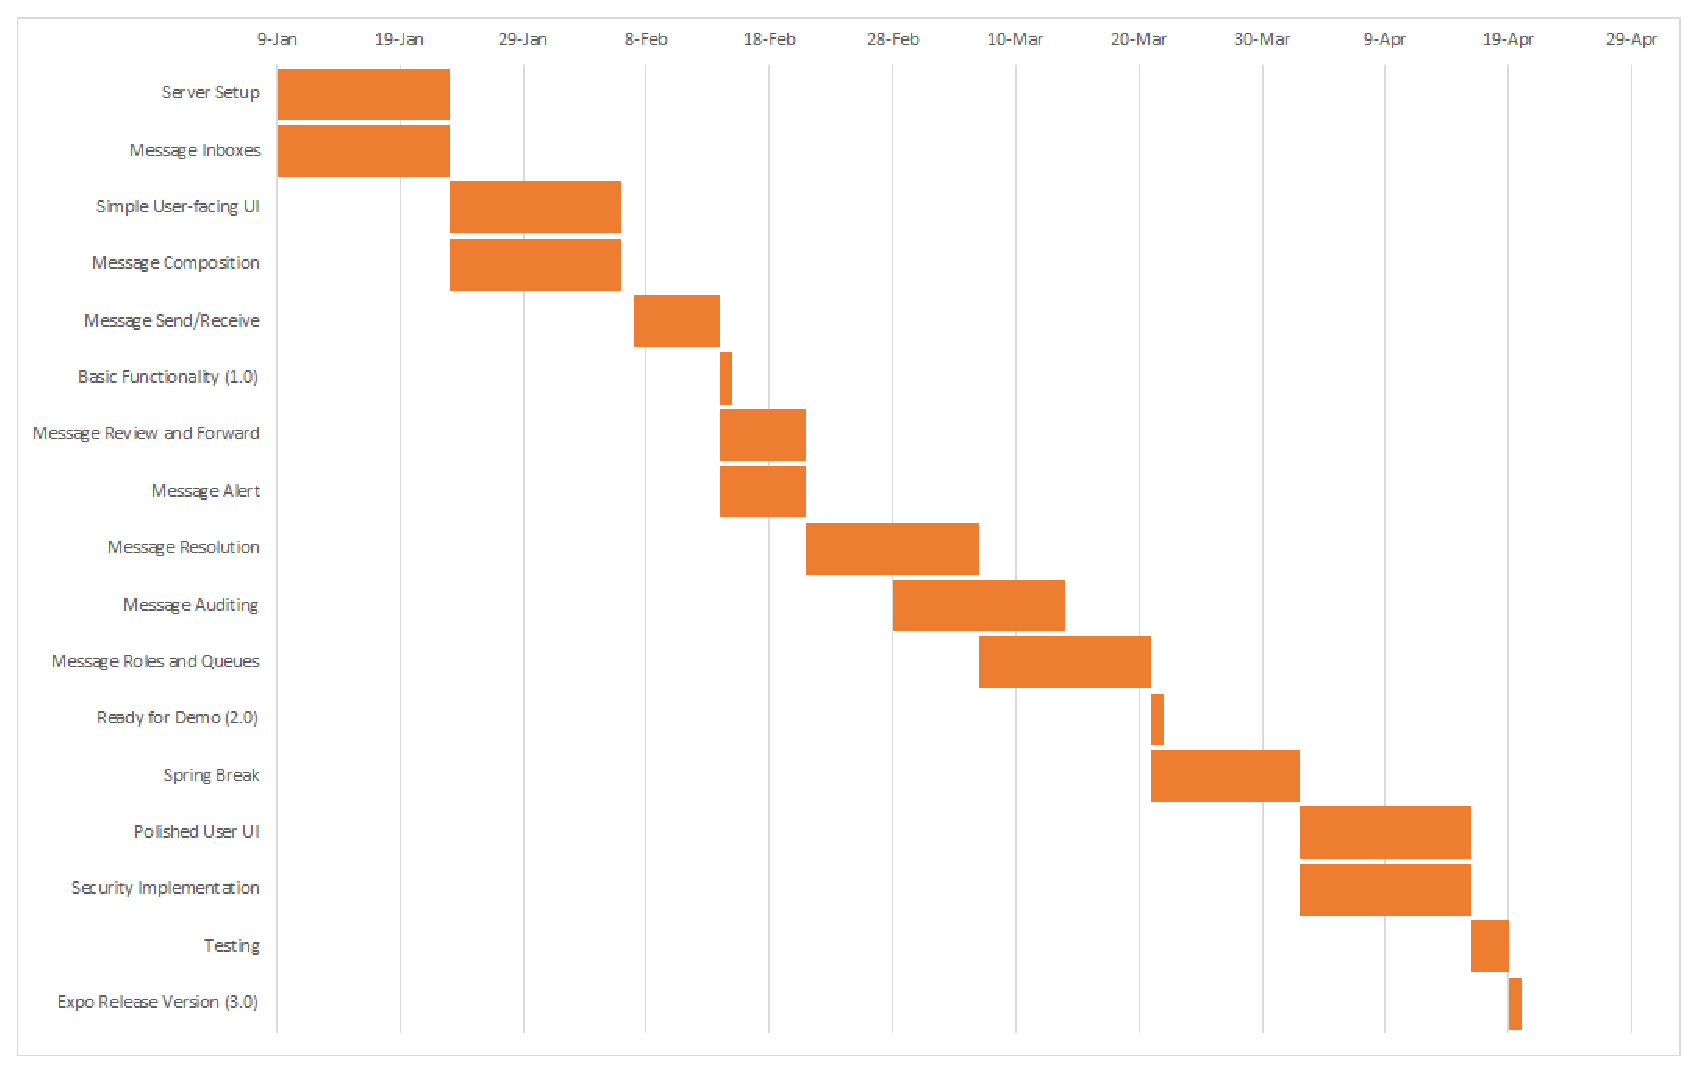
\includegraphics[angle=-90,origin=c,width=\textwidth,height=\textheight,keepaspectratio]{gantt-chart.eps}

\subsection{Changes}
As no more information about the VetHosp system was given to the development team, no integration with VetHosp was completed. In place of this the develpment team added an additional feature to allow messages to be exported to a PDF file that can then be uploaded into the VetHosp system. It was also decided that email notifications would be sufficient and sms messaging was not necessary.

\subsection{Final Gantt Chart}
\includegraphics[angle=-90,origin=c,width=\textwidth,height=\textheight,keepaspectratio]{final-gantt-chart.eps}

\newpage
\section{Design Document}



\subsection{Changes}

\newpage
\section{Tech Review}

\newpage
\section{Weekly Blog Posts}

\subsection{Henry}

\subsection{Kailyn}

\subsection{Taylor}

\newpage
\section{Final Poster}

\newpage
\section{Project Documentation}

\newpage
\section{Recommended Technical Resources for Learning More}
\subsection {Helpful Websites}
\begin{itemize}
\item https://docs.angularjs.org/guide/introduction
\item https://www.w3schools.com/
\item http://php.net/
\item https://dev.mysql.com/doc/
\end{itemize}

\newpage
\section{Conclusions and Reflections}

\subsection{Henry}

\subsubsection{What technical information did you learn?}

\subsubsection{What non-technical information did you learn?}

\subsubsection{What have you learned about project work?}

\subsubsection{What have you learned about project management?}

\subsubsection{What have you learned about working in teams?}

\subsubsection{If you could do it all over, what would you do differently?}

\subsection{Kailyn}

\subsubsection{What technical information did you learn?}

\subsubsection{What non-technical information did you learn?}

\subsubsection{What have you learned about project work?}

\subsubsection{What have you learned about project management?}

\subsubsection{What have you learned about working in teams?}

\subsubsection{If you could do it all over, what would you do differently?}

\subsection{Taylor}

\subsubsection{What technical information did you learn?}

\subsubsection{What non-technical information did you learn?}

\subsubsection{What have you learned about project work?}

\subsubsection{What have you learned about project management?}

\subsubsection{What have you learned about working in teams?}

\subsubsection{If you could do it all over, what would you do differently?}


\newpage
\section{Appendix 1: Essential Code Listings}

\newpage
\section{Appendix 2: Photos of Project}


\end{document}
